\subsection{SNMP Subagent implementation}
\label{section:sub-agent-implementation}
The SNMP subagent itself is based on the work of Pieter Hollants \cite{pythonnetsnmpagent} and provides us a Python API to communicate with the NET-SNMP master agent. The main function that updates the defined SNMP objects was implemented during the research project. That function uses the API calls shown in Table \ref{table:api-calls}.

\begin{table}[H]
	\centering
\begin{tabular}{|l|p{5.5cm}|}

\hline 
\textbf{API call} & \textbf{Description} \\ 
\hline 
\tt{tablename.clear} & clears a table row\\ 
\hline 
\tt{tablename.addRow} & adds a table row\\ 
\hline 
\tt{tablename.rowid.setRowCell} & sets a value to a cell in a table row\\ 
\hline 
\end{tabular} 
\caption{API calls python-netsnmpagent}
\label{table:api-calls}
\end{table}

The values that are assigned to object-type instances are derived from an XML data file. The function that implements the SNMP variables-update reads in the XML structure and iterates for all announced zones through the XML document using XPath queries \citep{xpath}. Everytime a corresponding table  entry is identified, that entry, and in turn the related SNMP variable get updated. The function is included in the \textit{agent} directory on Github \cite{github}. Figure \ref{figure:workflow} shows the  workflow of the function.

\begin{figure}[H]
\centering
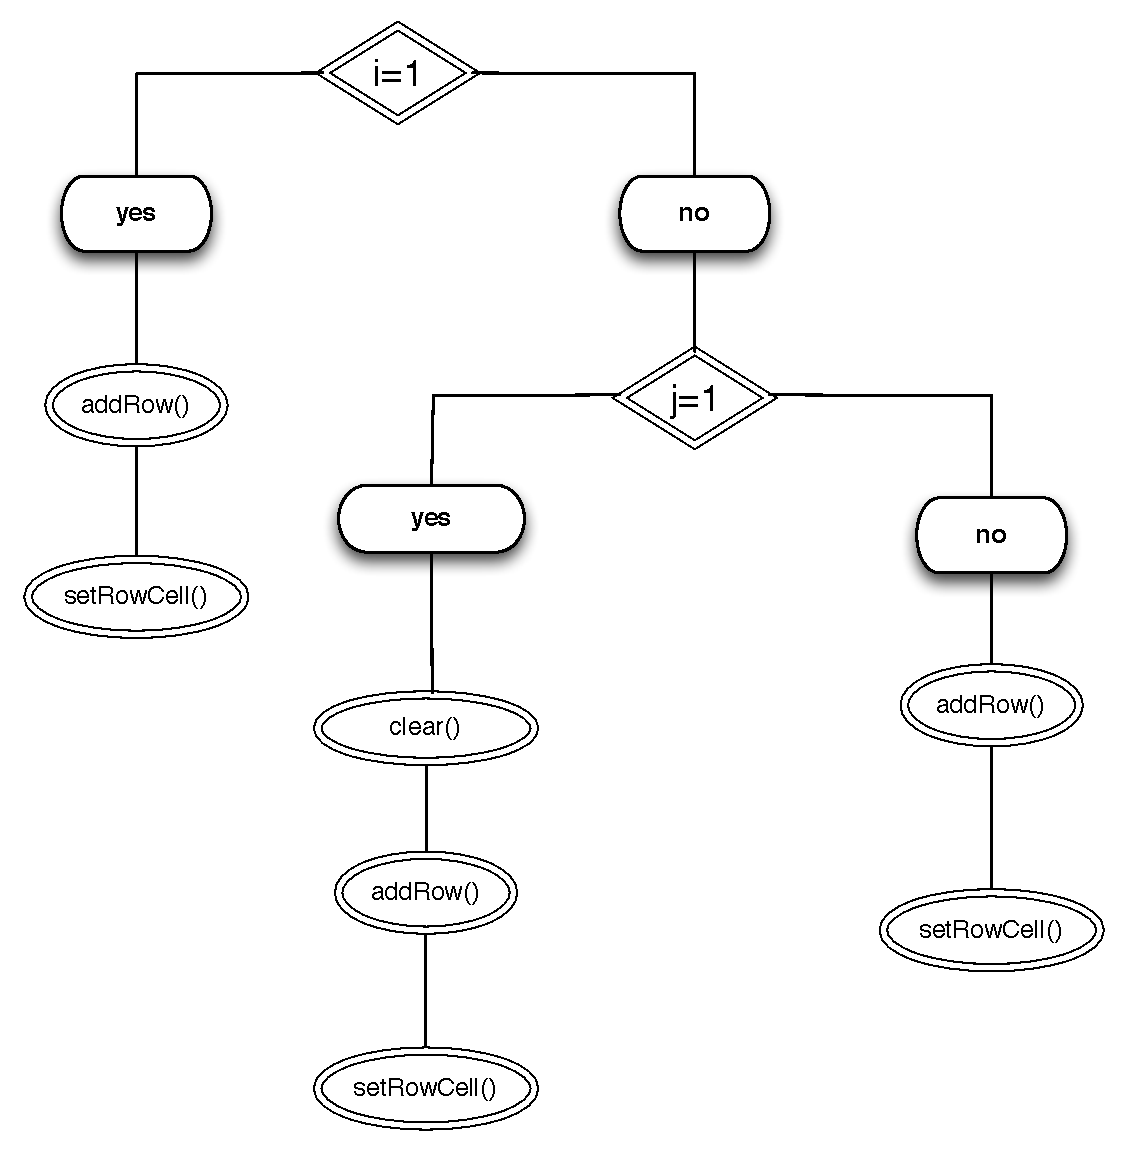
\includegraphics[scale=0.5]{Images/workflow.pdf}
\caption{workflow of the subagent's UpdateSNMPObjs() function}
\label{figure:workflow}
\end{figure}

The function first checks if it is executed the first time \textit{(i=1)}. If so, table rows are added instantly. The counter variable \textit{i} is incremented each time the function is called. If \textit{i} is not equal to one, another counter variable \textit{j} is checked. That counter indicates which round of iteration is currently performed inside the function. Only, and only if it is the first iteration, the current table is cleared and after that new values are added.
\\
The SNMP subagent operates asynchronously. The data update thread is decoupled from the data providing thread. This ensures periodic data updates and also makes sure that SNMP requests will always be answered to in time. Zones can be added or removed dynamically by specifying them in the \textit{zone\_hint} file. Figure \ref{figure:subagent} shows the interaction between all components that are involved.

\begin{figure}[H]
\centering
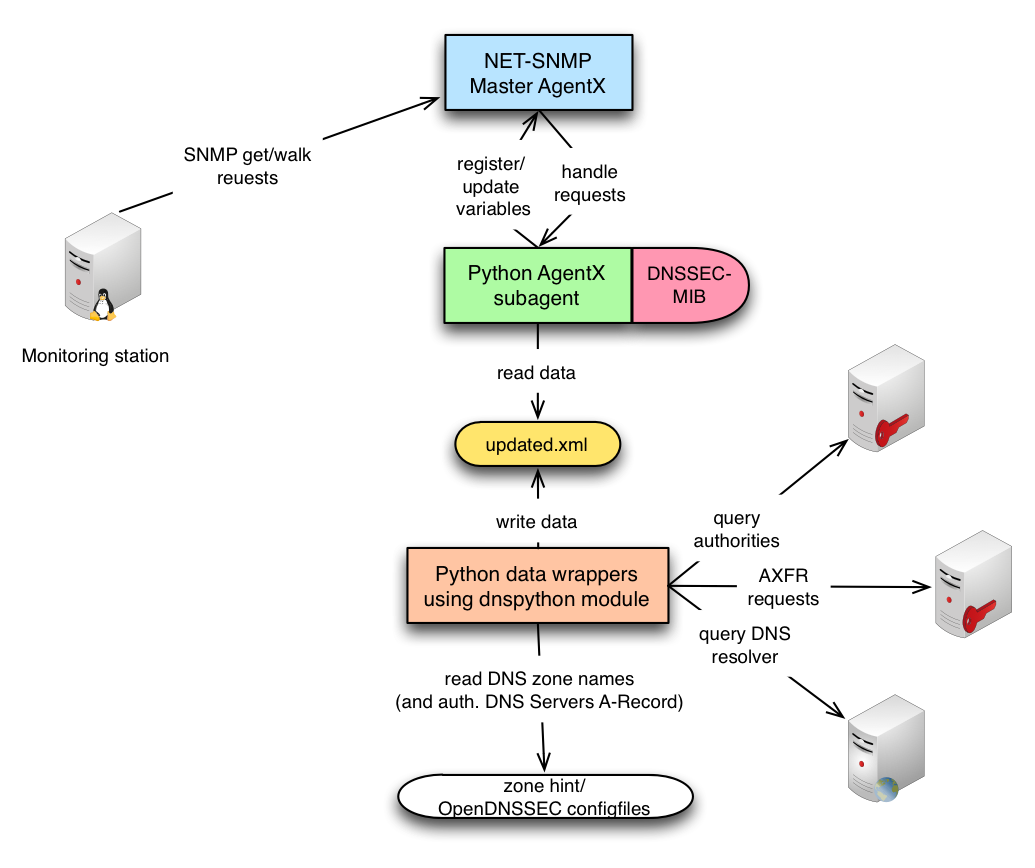
\includegraphics[scale=0.7]{Images/topology3.pdf}
\caption{logical scheme SNMP subagent}
\label{figure:subagent}
\end{figure}
 
